\chapter{Introduction}
\section{General Knowledge of DDoS}
Distributed Denial of Service (DDoS) attacks are currently one of the most dangerous and threatening phenomena for the modern network. A Distributed Denial of Service (DDoS) attack is an attempt to make a service unavailable by overwhelming the server with malicious traffic \cite{8394146}. This disrupts the normal flow of operations; it makes some services unattainable to genuine customers. Traditionally, DoS attackers target the server, which is providing a service to its consumers. Behaving like a legitimate customer, DoS attackers try to flood active server in a manner such that the service becomes unavailable due to a large number of requests pending and overflowing the service queue. A different flavor of DoS is Distributed DoS, or DDoS, where attackers are a group of machines targeting a particular service \cite{somani2017ddos}. While a regular DoS attack comes from a single source, a DDoS attack involves the use of several network elements, known as a botnet. They are used secretly to enhance the ferocity of the attack against the ownership of the devise. Different technical methods can be used by DDoS attackers to disrupt regular service operations. The server faces excessive work along with extensive bandwidth utilization that serves as the primary targets of DDoS attacks.All forms of network data can be used to consume bandwidth. The main traffic sent by DDoS attackers will be identical throughout all their zombie systems. ICMP Echo Request floods serve as the most frequent attack vector under the "ping" flood moniker, while other traffic types such as UDP or TCP also function for this purpose \cite{NAZARIO20087}. \\
An attack involving Denial of Service disables network resources. The attack surface exposed through DDoS attacks spans a wide range. The Total number of hardware and software items linked to the internet constitutes the basic definition of network infrastructure. This includes:
\\
• Network resources (hubs, routers, firewalls, gateways, wireless spectrum, etc.),\\
• System resources (computer memory, network interfaces, operating systems, web servers, etc.),\\
• Protocol definitions and implementations, and \\
• Physical damage (cables, optical cables, power lines, satellites, etc.) \cite{ozccelik2020distributed}
\newpage
\begin{figure}[!htb]
    \centering
    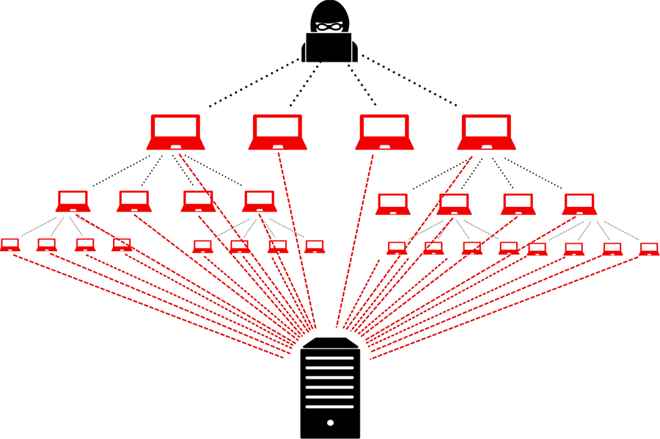
\includegraphics[scale=0.6]{thesis/ddos.png}
    \caption{DDoS attack}
    \label{fig:enter-label}
\end{figure}
\section{Evolution of DDoS}
\\In 1988 Morris worm malware pioneered the first DDoS attack after it infected at least 60,000 nodes \cite{fazio2020packet}. Evidence shows that the first officially documented DDoS attack developed by Cyber Emergency Response Team (CERT) emerged ten years after the initial attacks in 1998 and became known as Smurf \cite{abubakar2020effective,goswami2021probability}. Unexpected access led to various problems for victims who experienced both customer loss and decreased credibility together with financial challenges and system downtime as direct consequences \cite{sundarapandian2009probability}. DoS and DDoS attacks are increasing rapidly both in frequency and intensity with an average of 28.7K attacks per day \cite{MANSFIELDDEVINE201513,MANSFIELDDEVINE201514}. Recently, Neustar's report on cyber threats and trends \cite{jonker2017millions} revealed that DDoS attacks have increased 200\% in frequency while 73\% increased in volume during the first six months of 2019 compared to the same period in 2018 \cite{threatstrends}.
\\
\begin{figure}[!htb]
    \centering
    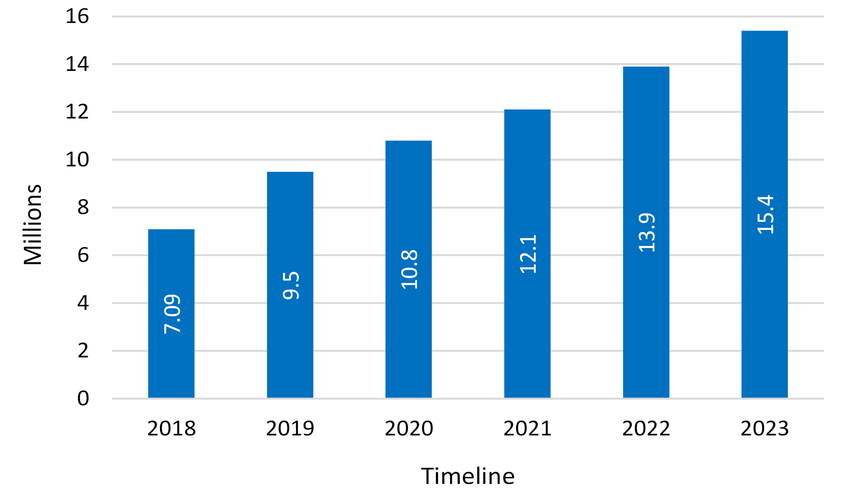
\includegraphics[width=0.8\linewidth]{thesis/timeline.png}
    \caption{ Global Trend of DDoS Attacks 2018-2023}
    \label{fig:enter-label}
\end{figure}
\newpage
\section{Networking Background}
The world became permeated by the Internet because of accelerating technological progress. The improvement of access speeds combined with growing access reliability leads to diverse Internet services that influence every aspect of daily life. People depend daily on Internet services for transmitting confidential as well as professional and personal data between themselves. People use inherent Internet weaknesses to halt services across the entire network since society requires constant Internet operations. The analysis of unwanted network intrusions has evolved into an essential research topic because network attack incidents continue to rise \cite{unknown}. 
\\
\begin{figure}[!htb]
    \centering
    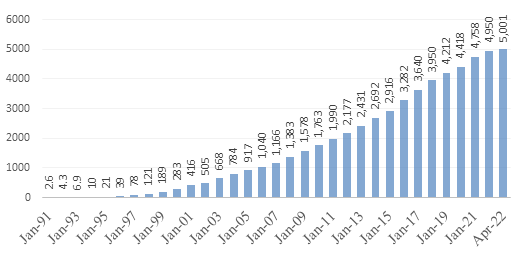
\includegraphics[width=0.8\linewidth]{thesis/internetUser.png}
    \caption{Number of Internet users worldwide in billion from January of the year 1991 until the month of April of the year 2022 \cite{bhattacharyya2016ddos}}
    \label{fig:enter-label}
\end{figure}
\section{GNS-3 Background}
GNS3 which stands for Graphical Network Simulator 3, it functions as an emulation platform to simulate network devices that can connect routers with firewalls and switches and multiple other devices that work within the OSI model \cite{article}. GNS3 enables users to design network labs that precisely match their requirements while supporting endless projects that combine Cisco and other vendor technologies alongside unrestricted object additions and project availability at any time without requiring Internet. Through a combination of real network operating system running on emulated hardware devices and simulated operating systems and multiple computer resource sharing GNS3 delivers maximum design flexibility \cite{fomin2017gns3}. Actually, GNS3 allows for emulation of different types of networking protocols, giving the practical opportunity to make configuration and study traffic flow. It also successfully addresses issues related to the visualisation of the network that is so important for cyber security research. Hence, the researchers can model live networks through the GNS3, whereby different scenarios such as DOS can be created in order to identify the weaknesses and strength of different solutions before they are implemented on the live network. Users can then interact with their simulated networks, monitor traffic with tools like Wireshark, and troubleshoot issues in real-time. Furthermore, GNS3 offers extensive support for network automation and scripting through integration with tools like Ansible and Python. This enables users to deploy configurations across multiple devices efficiently \cite{neumann2015book}.
\begin{figure}[!htb]
    \centering
    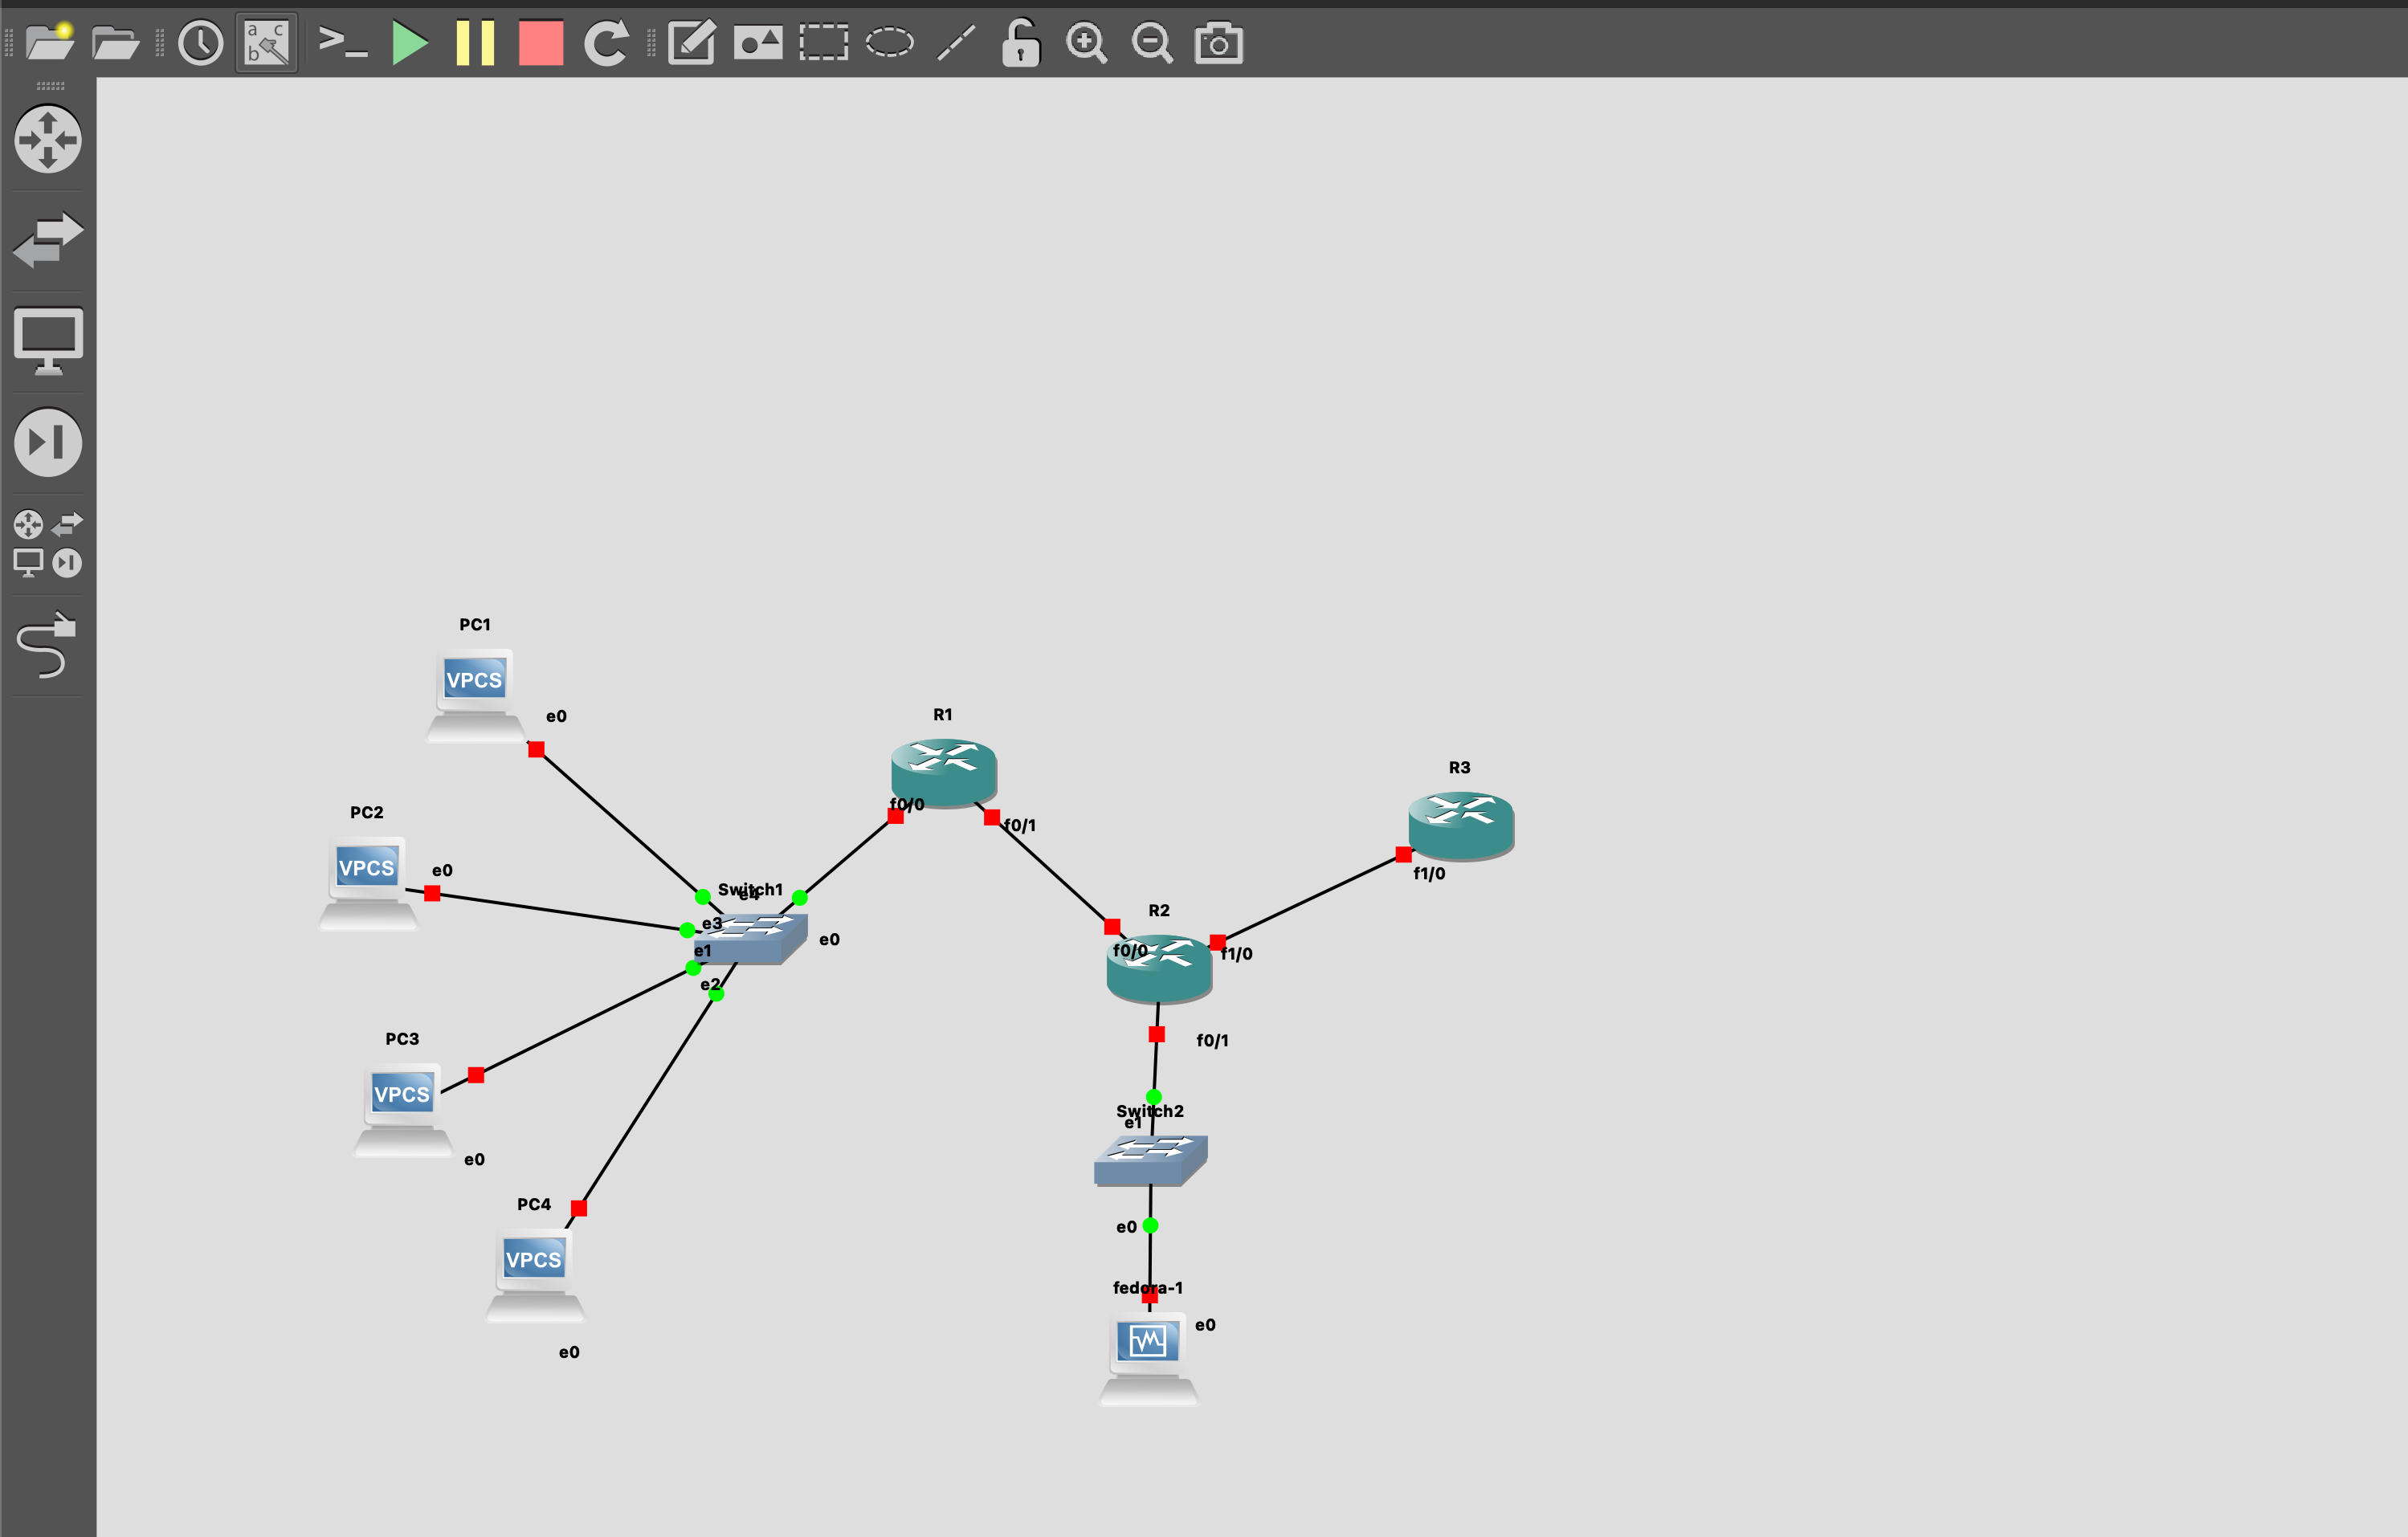
\includegraphics[width=0.8\linewidth]{thesis/gns3.png}
    \caption{GNS-3 interface}
    \label{fig:enter-label}
\end{figure}
\section{Suricata Information}
One of the threats in the digital environment today is network-based attacks like Distributed Denial of Service (DDoS) attacks which can cause serious malice to the availability, secrecy, and privacy of key systems. Due to the increasing and advanced nature of cyberattacks, there has been a notable increase in the need of effective/strong real-time security mechanisms. The sheer number of network defense tools on the market makes it quite difficult to select which one to use, and Suricata is an open-source high-performance tool that can easily be used as an Intrusion Detection System (IDS), an Intrusion Prevention System (IPS) and as a network security monitoring engine \cite{veerasingam2023intrusion}.
\\
The network-based IDS/IPS accounted for a share of over 24\% in 2018 in the global intrusion detection system / intrusion prevention system market, BFSI is expected to grow in terms of CAGR with the highest velocity i.e., 15\% in the IDS/IPS market in 2019, 2025 \cite{gminsights}. 
\pagebreak
\begin{figure}[!htb]
    \centering
    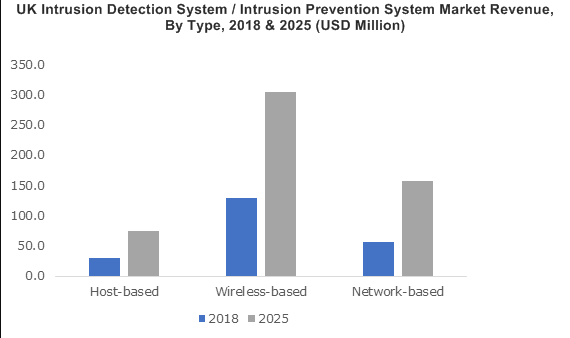
\includegraphics[width=0.8\linewidth]{thesis/ipsStats.png}
    \caption{UK IPS/IDS revenue market}
    \label{fig:enter-label}
\end{figure}
\\
Suricata is scalable to view network traffic in deep details with the help of signature-based detection rules and anomaly-based behavior analysis \cite{inbook}. Where older intrusion detection tools were based on linear progression and could only work at a relatively slow pace on network packets, Suricata uses multi-threading and other hardware optimizations to work in conjunction with a vast number of network messages \cite{article1}. It also allows more advanced capabilities like file extraction, TLS and Apache HTTP inspection, scripting via Lua and output standardizing to other security systems via standard output formats like EVE JSON. In this project, we configure NFQ and iptables to accept or drop the incoming packets.
\begin{figure}[!htb]
    \centering
    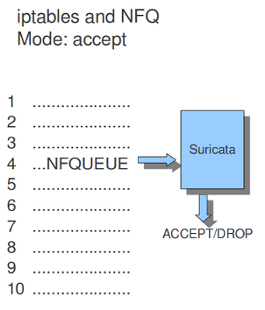
\includegraphics[scale=0.6]{thesis/suricataMode.png}
    \caption{NFQUEUE in iptables rules}
    \label{fig:enter-label}
\end{figure}
\newline
Deep packet inspection Suricata has been designed around the idea of deep packet inspection (DPI) \cite{chandramouli2025advanced}. Suricata as an IDS transports traffic and creates alerts of suspicious activity depending on compiled rules. It is even more proactive in IPS mode, where it is able to drop or change packet in real time to stop malicious traffic. Depending on the deployment and network architecture, Suricata has the ability to run in many different run modes which include, but are not limited to, AF\_PACKET, NFQUEUE or PCAP.
\\
This thesis examines how Suricata is effective and functional in identifying and countering UDP-based DDoS attacks in a simulated area with GNS3. This research seeks to test the ability of this tool in offering protection in real time and presence of services by profiling the network behavior in different attack conditions with Suricata configured in IPS mode. Moreover, it uses Wireshark and Suricata logs, so as to visualize and evaluate traffic before and after IPS implementation.
\section{Problem Statement}
System and network administration training requires intensive hands-on practice. In order to ease the financial implication and at the same time aiming to help all the people get hands-on practice, the system and network administration practical lessons were conducted in a simulated network environment with the help of Graphical Network Simulator (GNS3) to emulate the devices such as servers, switches, routers, etc \cite{azem2024network}.
\section{Motivation and Objectives}
\subsection{Motivation}
The motivation for this thesis lies in rising and escalating threat of Distributed Denial of Service (DDoS) attacks that endanger freedom of access to connections in the contemporary interconnected world. Since organizations and individuals are now using the Internet in many sensitive activities, the effects of such attacks are more severe as they result in losses, reputations losses and interruption of services. The increasing use of IoT devices has also extended the threat level; the gadgets in the range are generally not very secure and allow attackers to create an extensive botnet for further use.
\\
In that regard, current advances of cybersecurity studies still present a severe dearth of effective knowledge on DDoS attacks and its types across different network environments and the efficacy of protective measures. It is therefore important to model such attacks in a contained setting in order to study their effects, find weaknesses and analyze potential counter measures.
\\
This thesis is fueled by the fact that GNS3 (Graphical Network Simulator–3) a powerful and cost-effective emulation platform for computer networks. This feature is unique in the fact that it offers the user the chance to create topologies and experiment on them using only the software without having to use any physical hardware. Using GNS3, this study aims at presenting to the body of knowledge in cybersecurity an understanding of the behaviours of DDoS attacks as well as a potential approach to their prevention in virtual network.
\subsection{Objecetives}
Based on the above background, this thesis aims to utilize GNS3 to set up a Virtual Network and perform analysis on DDoS and its impacts with regard to the development of countermeasures. The specific objectives include:
\begin{itemize}
\item Architecture of a Virtual Network and Its Integration in the GNS3
\\
Establish a flow that connects main parts of communication system like routers, switches, servers and client devices.
Make sure that all the traffic on the network resembles live situation and the devices’ settings were accurately recreated.
\item Simulation of DDoS Attacks
\\
The techniques employed when planning a simulation should be able to cover various classes of DDoS attacks, which are; the volumetric attacks, the protocol attacks and the application layer attacks.Compare the results of these attacks with traditional generic network performance parameters including bandwidth usage, delay, and loss rate.
\item Analysis of Attack Behavior
Keep a record of the behavior of all the significant components of the network during a DDoS attack.
Describe weaknesses and passing obstacles taken advantage of by the attacks.
\item Assessment of Risk Reduction Measures
Many different defences can be put in place and tested such as rate limiting, firewalls, and intrusion detection/prevention systems. Evaluating the effectiveness of these strategies towards minimizing the effect of DDoS attacks.
\item Stand for Developing Cybersecurity Information
Be useful for network engineers and researchers and include realistic proposals and observations.
Emphasize the strength and weaknesses of GNS3 for emulating and analyzing the performances of the class-based DDoS philtres.
\end{itemize}
\\
Thus, the following objectives have been laid down for this research; Through these objectives, this research hopes to contribute positively towards reducing the gap between theoretical development and realistic implementation and implementation of effective measures that can be used by the stakeholders in order to minimize the impacts of DDoS threats.